% Created by tikzDevice version 0.12
% !TEX encoding = UTF-8 Unicode
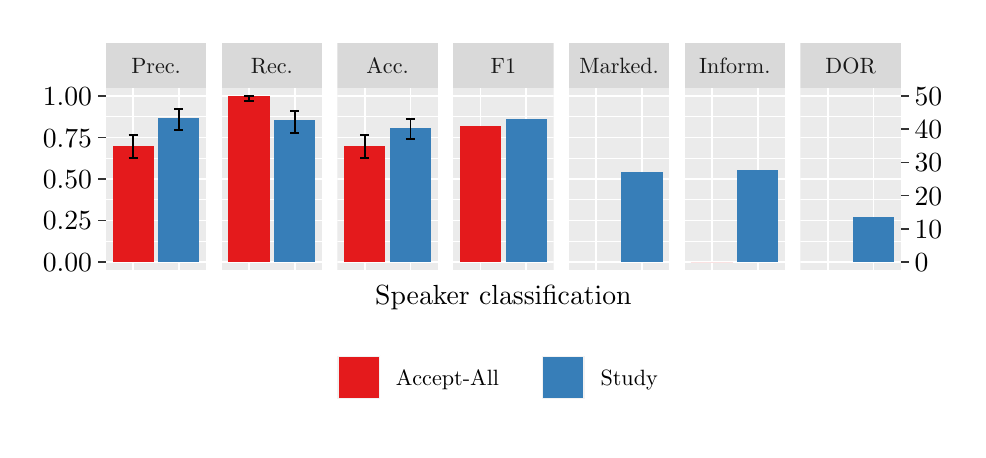
\begin{tikzpicture}[x=1pt,y=1pt]
\definecolor{fillColor}{RGB}{255,255,255}
\path[use as bounding box,fill=fillColor,fill opacity=0.00] (0,0) rectangle (336.00,145.35);
\begin{scope}
\path[clip] (  0.00,  0.00) rectangle (336.00,145.35);
\definecolor{drawColor}{RGB}{255,255,255}
\definecolor{fillColor}{RGB}{255,255,255}

\path[draw=drawColor,line width= 0.6pt,line join=round,line cap=round,fill=fillColor] (  0.00,  0.00) rectangle (336.00,145.35);
\end{scope}
\begin{scope}
\path[clip] ( 28.22, 57.73) rectangle ( 64.56,123.60);
\definecolor{fillColor}{gray}{0.92}

\path[fill=fillColor] ( 28.22, 57.73) rectangle ( 64.56,123.60);
\definecolor{drawColor}{RGB}{255,255,255}

\path[draw=drawColor,line width= 0.3pt,line join=round] ( 28.22, 68.21) --
	( 64.56, 68.21);

\path[draw=drawColor,line width= 0.3pt,line join=round] ( 28.22, 83.18) --
	( 64.56, 83.18);

\path[draw=drawColor,line width= 0.3pt,line join=round] ( 28.22, 98.15) --
	( 64.56, 98.15);

\path[draw=drawColor,line width= 0.3pt,line join=round] ( 28.22,113.12) --
	( 64.56,113.12);

\path[draw=drawColor,line width= 0.6pt,line join=round] ( 28.22, 60.72) --
	( 64.56, 60.72);

\path[draw=drawColor,line width= 0.6pt,line join=round] ( 28.22, 75.69) --
	( 64.56, 75.69);

\path[draw=drawColor,line width= 0.6pt,line join=round] ( 28.22, 90.67) --
	( 64.56, 90.67);

\path[draw=drawColor,line width= 0.6pt,line join=round] ( 28.22,105.64) --
	( 64.56,105.64);

\path[draw=drawColor,line width= 0.6pt,line join=round] ( 28.22,120.61) --
	( 64.56,120.61);

\path[draw=drawColor,line width= 0.6pt,line join=round] ( 38.13, 57.73) --
	( 38.13,123.60);

\path[draw=drawColor,line width= 0.6pt,line join=round] ( 54.65, 57.73) --
	( 54.65,123.60);
\definecolor{fillColor}{RGB}{228,26,28}

\path[fill=fillColor] ( 30.70, 60.72) rectangle ( 45.56,102.57);
\definecolor{fillColor}{RGB}{55,126,184}

\path[fill=fillColor] ( 47.22, 60.72) rectangle ( 62.08,112.69);
\definecolor{drawColor}{RGB}{0,0,0}

\path[draw=drawColor,line width= 0.6pt,line join=round] ( 53.00,115.96) --
	( 56.30,115.96);

\path[draw=drawColor,line width= 0.6pt,line join=round] ( 54.65,115.96) --
	( 54.65,108.28);

\path[draw=drawColor,line width= 0.6pt,line join=round] ( 53.00,108.28) --
	( 56.30,108.28);

\path[draw=drawColor,line width= 0.6pt,line join=round] ( 36.48,106.57) --
	( 39.78,106.57);

\path[draw=drawColor,line width= 0.6pt,line join=round] ( 38.13,106.57) --
	( 38.13, 98.17);

\path[draw=drawColor,line width= 0.6pt,line join=round] ( 36.48, 98.17) --
	( 39.78, 98.17);
\end{scope}
\begin{scope}
\path[clip] ( 70.06, 57.73) rectangle (106.39,123.60);
\definecolor{fillColor}{gray}{0.92}

\path[fill=fillColor] ( 70.06, 57.73) rectangle (106.39,123.60);
\definecolor{drawColor}{RGB}{255,255,255}

\path[draw=drawColor,line width= 0.3pt,line join=round] ( 70.06, 68.21) --
	(106.39, 68.21);

\path[draw=drawColor,line width= 0.3pt,line join=round] ( 70.06, 83.18) --
	(106.39, 83.18);

\path[draw=drawColor,line width= 0.3pt,line join=round] ( 70.06, 98.15) --
	(106.39, 98.15);

\path[draw=drawColor,line width= 0.3pt,line join=round] ( 70.06,113.12) --
	(106.39,113.12);

\path[draw=drawColor,line width= 0.6pt,line join=round] ( 70.06, 60.72) --
	(106.39, 60.72);

\path[draw=drawColor,line width= 0.6pt,line join=round] ( 70.06, 75.69) --
	(106.39, 75.69);

\path[draw=drawColor,line width= 0.6pt,line join=round] ( 70.06, 90.67) --
	(106.39, 90.67);

\path[draw=drawColor,line width= 0.6pt,line join=round] ( 70.06,105.64) --
	(106.39,105.64);

\path[draw=drawColor,line width= 0.6pt,line join=round] ( 70.06,120.61) --
	(106.39,120.61);

\path[draw=drawColor,line width= 0.6pt,line join=round] ( 79.97, 57.73) --
	( 79.97,123.60);

\path[draw=drawColor,line width= 0.6pt,line join=round] ( 96.48, 57.73) --
	( 96.48,123.60);
\definecolor{fillColor}{RGB}{228,26,28}

\path[fill=fillColor] ( 72.53, 60.72) rectangle ( 87.40,120.61);
\definecolor{fillColor}{RGB}{55,126,184}

\path[fill=fillColor] ( 89.05, 60.72) rectangle (103.91,111.84);
\definecolor{drawColor}{RGB}{0,0,0}

\path[draw=drawColor,line width= 0.6pt,line join=round] ( 94.83,115.27) --
	( 98.13,115.27);

\path[draw=drawColor,line width= 0.6pt,line join=round] ( 96.48,115.27) --
	( 96.48,107.35);

\path[draw=drawColor,line width= 0.6pt,line join=round] ( 94.83,107.35) --
	( 98.13,107.35);

\path[draw=drawColor,line width= 0.6pt,line join=round] ( 78.31,120.61) --
	( 81.62,120.61);

\path[draw=drawColor,line width= 0.6pt,line join=round] ( 79.97,120.61) --
	( 79.97,118.84);

\path[draw=drawColor,line width= 0.6pt,line join=round] ( 78.31,118.84) --
	( 81.62,118.84);
\end{scope}
\begin{scope}
\path[clip] (111.89, 57.73) rectangle (148.22,123.60);
\definecolor{fillColor}{gray}{0.92}

\path[fill=fillColor] (111.89, 57.73) rectangle (148.22,123.60);
\definecolor{drawColor}{RGB}{255,255,255}

\path[draw=drawColor,line width= 0.3pt,line join=round] (111.89, 68.21) --
	(148.22, 68.21);

\path[draw=drawColor,line width= 0.3pt,line join=round] (111.89, 83.18) --
	(148.22, 83.18);

\path[draw=drawColor,line width= 0.3pt,line join=round] (111.89, 98.15) --
	(148.22, 98.15);

\path[draw=drawColor,line width= 0.3pt,line join=round] (111.89,113.12) --
	(148.22,113.12);

\path[draw=drawColor,line width= 0.6pt,line join=round] (111.89, 60.72) --
	(148.22, 60.72);

\path[draw=drawColor,line width= 0.6pt,line join=round] (111.89, 75.69) --
	(148.22, 75.69);

\path[draw=drawColor,line width= 0.6pt,line join=round] (111.89, 90.67) --
	(148.22, 90.67);

\path[draw=drawColor,line width= 0.6pt,line join=round] (111.89,105.64) --
	(148.22,105.64);

\path[draw=drawColor,line width= 0.6pt,line join=round] (111.89,120.61) --
	(148.22,120.61);

\path[draw=drawColor,line width= 0.6pt,line join=round] (121.80, 57.73) --
	(121.80,123.60);

\path[draw=drawColor,line width= 0.6pt,line join=round] (138.31, 57.73) --
	(138.31,123.60);
\definecolor{fillColor}{RGB}{228,26,28}

\path[fill=fillColor] (114.37, 60.72) rectangle (129.23,102.57);
\definecolor{fillColor}{RGB}{55,126,184}

\path[fill=fillColor] (130.88, 60.72) rectangle (145.74,109.04);
\definecolor{drawColor}{RGB}{0,0,0}

\path[draw=drawColor,line width= 0.6pt,line join=round] (136.66,112.36) --
	(139.96,112.36);

\path[draw=drawColor,line width= 0.6pt,line join=round] (138.31,112.36) --
	(138.31,105.08);

\path[draw=drawColor,line width= 0.6pt,line join=round] (136.66,105.08) --
	(139.96,105.08);

\path[draw=drawColor,line width= 0.6pt,line join=round] (120.15,106.57) --
	(123.45,106.57);

\path[draw=drawColor,line width= 0.6pt,line join=round] (121.80,106.57) --
	(121.80, 98.17);

\path[draw=drawColor,line width= 0.6pt,line join=round] (120.15, 98.17) --
	(123.45, 98.17);
\end{scope}
\begin{scope}
\path[clip] (153.72, 57.73) rectangle (190.05,123.60);
\definecolor{fillColor}{gray}{0.92}

\path[fill=fillColor] (153.72, 57.73) rectangle (190.05,123.60);
\definecolor{drawColor}{RGB}{255,255,255}

\path[draw=drawColor,line width= 0.3pt,line join=round] (153.72, 68.21) --
	(190.05, 68.21);

\path[draw=drawColor,line width= 0.3pt,line join=round] (153.72, 83.18) --
	(190.05, 83.18);

\path[draw=drawColor,line width= 0.3pt,line join=round] (153.72, 98.15) --
	(190.05, 98.15);

\path[draw=drawColor,line width= 0.3pt,line join=round] (153.72,113.12) --
	(190.05,113.12);

\path[draw=drawColor,line width= 0.6pt,line join=round] (153.72, 60.72) --
	(190.05, 60.72);

\path[draw=drawColor,line width= 0.6pt,line join=round] (153.72, 75.69) --
	(190.05, 75.69);

\path[draw=drawColor,line width= 0.6pt,line join=round] (153.72, 90.67) --
	(190.05, 90.67);

\path[draw=drawColor,line width= 0.6pt,line join=round] (153.72,105.64) --
	(190.05,105.64);

\path[draw=drawColor,line width= 0.6pt,line join=round] (153.72,120.61) --
	(190.05,120.61);

\path[draw=drawColor,line width= 0.6pt,line join=round] (163.63, 57.73) --
	(163.63,123.60);

\path[draw=drawColor,line width= 0.6pt,line join=round] (180.15, 57.73) --
	(180.15,123.60);
\definecolor{fillColor}{RGB}{228,26,28}

\path[fill=fillColor] (156.20, 60.72) rectangle (171.06,109.99);
\definecolor{fillColor}{RGB}{55,126,184}

\path[fill=fillColor] (172.71, 60.72) rectangle (187.58,112.26);
\end{scope}
\begin{scope}
\path[clip] (195.55, 57.73) rectangle (231.89,123.60);
\definecolor{fillColor}{gray}{0.92}

\path[fill=fillColor] (195.55, 57.73) rectangle (231.89,123.60);
\definecolor{drawColor}{RGB}{255,255,255}

\path[draw=drawColor,line width= 0.3pt,line join=round] (195.55, 68.21) --
	(231.89, 68.21);

\path[draw=drawColor,line width= 0.3pt,line join=round] (195.55, 83.18) --
	(231.89, 83.18);

\path[draw=drawColor,line width= 0.3pt,line join=round] (195.55, 98.15) --
	(231.89, 98.15);

\path[draw=drawColor,line width= 0.3pt,line join=round] (195.55,113.12) --
	(231.89,113.12);

\path[draw=drawColor,line width= 0.6pt,line join=round] (195.55, 60.72) --
	(231.89, 60.72);

\path[draw=drawColor,line width= 0.6pt,line join=round] (195.55, 75.69) --
	(231.89, 75.69);

\path[draw=drawColor,line width= 0.6pt,line join=round] (195.55, 90.67) --
	(231.89, 90.67);

\path[draw=drawColor,line width= 0.6pt,line join=round] (195.55,105.64) --
	(231.89,105.64);

\path[draw=drawColor,line width= 0.6pt,line join=round] (195.55,120.61) --
	(231.89,120.61);

\path[draw=drawColor,line width= 0.6pt,line join=round] (205.46, 57.73) --
	(205.46,123.60);

\path[draw=drawColor,line width= 0.6pt,line join=round] (221.98, 57.73) --
	(221.98,123.60);
\definecolor{fillColor}{RGB}{55,126,184}

\path[fill=fillColor] (214.55, 60.72) rectangle (229.41, 93.09);
\end{scope}
\begin{scope}
\path[clip] (237.39, 57.73) rectangle (273.72,123.60);
\definecolor{fillColor}{gray}{0.92}

\path[fill=fillColor] (237.39, 57.73) rectangle (273.72,123.60);
\definecolor{drawColor}{RGB}{255,255,255}

\path[draw=drawColor,line width= 0.3pt,line join=round] (237.39, 68.21) --
	(273.72, 68.21);

\path[draw=drawColor,line width= 0.3pt,line join=round] (237.39, 83.18) --
	(273.72, 83.18);

\path[draw=drawColor,line width= 0.3pt,line join=round] (237.39, 98.15) --
	(273.72, 98.15);

\path[draw=drawColor,line width= 0.3pt,line join=round] (237.39,113.12) --
	(273.72,113.12);

\path[draw=drawColor,line width= 0.6pt,line join=round] (237.39, 60.72) --
	(273.72, 60.72);

\path[draw=drawColor,line width= 0.6pt,line join=round] (237.39, 75.69) --
	(273.72, 75.69);

\path[draw=drawColor,line width= 0.6pt,line join=round] (237.39, 90.67) --
	(273.72, 90.67);

\path[draw=drawColor,line width= 0.6pt,line join=round] (237.39,105.64) --
	(273.72,105.64);

\path[draw=drawColor,line width= 0.6pt,line join=round] (237.39,120.61) --
	(273.72,120.61);

\path[draw=drawColor,line width= 0.6pt,line join=round] (247.30, 57.73) --
	(247.30,123.60);

\path[draw=drawColor,line width= 0.6pt,line join=round] (263.81, 57.73) --
	(263.81,123.60);
\definecolor{fillColor}{RGB}{228,26,28}

\path[fill=fillColor] (239.86, 60.72) rectangle (254.73, 60.72);
\definecolor{fillColor}{RGB}{55,126,184}

\path[fill=fillColor] (256.38, 60.72) rectangle (271.24, 93.77);
\end{scope}
\begin{scope}
\path[clip] (279.22, 57.73) rectangle (315.55,123.60);
\definecolor{fillColor}{gray}{0.92}

\path[fill=fillColor] (279.22, 57.73) rectangle (315.55,123.60);
\definecolor{drawColor}{RGB}{255,255,255}

\path[draw=drawColor,line width= 0.3pt,line join=round] (279.22, 68.21) --
	(315.55, 68.21);

\path[draw=drawColor,line width= 0.3pt,line join=round] (279.22, 83.18) --
	(315.55, 83.18);

\path[draw=drawColor,line width= 0.3pt,line join=round] (279.22, 98.15) --
	(315.55, 98.15);

\path[draw=drawColor,line width= 0.3pt,line join=round] (279.22,113.12) --
	(315.55,113.12);

\path[draw=drawColor,line width= 0.6pt,line join=round] (279.22, 60.72) --
	(315.55, 60.72);

\path[draw=drawColor,line width= 0.6pt,line join=round] (279.22, 75.69) --
	(315.55, 75.69);

\path[draw=drawColor,line width= 0.6pt,line join=round] (279.22, 90.67) --
	(315.55, 90.67);

\path[draw=drawColor,line width= 0.6pt,line join=round] (279.22,105.64) --
	(315.55,105.64);

\path[draw=drawColor,line width= 0.6pt,line join=round] (279.22,120.61) --
	(315.55,120.61);

\path[draw=drawColor,line width= 0.6pt,line join=round] (289.13, 57.73) --
	(289.13,123.60);

\path[draw=drawColor,line width= 0.6pt,line join=round] (305.64, 57.73) --
	(305.64,123.60);
\definecolor{fillColor}{RGB}{55,126,184}

\path[fill=fillColor] (298.21, 60.72) rectangle (313.08, 76.88);
\end{scope}
\begin{scope}
\path[clip] ( 28.22,123.60) rectangle ( 64.56,139.85);
\definecolor{fillColor}{gray}{0.85}

\path[fill=fillColor] ( 28.22,123.60) rectangle ( 64.56,139.85);
\definecolor{drawColor}{gray}{0.10}

\node[text=drawColor,anchor=base,inner sep=0pt, outer sep=0pt, scale=  0.80] at ( 46.39,128.97) {Prec.};
\end{scope}
\begin{scope}
\path[clip] ( 70.06,123.60) rectangle (106.39,139.85);
\definecolor{fillColor}{gray}{0.85}

\path[fill=fillColor] ( 70.06,123.60) rectangle (106.39,139.85);
\definecolor{drawColor}{gray}{0.10}

\node[text=drawColor,anchor=base,inner sep=0pt, outer sep=0pt, scale=  0.80] at ( 88.22,128.97) {Rec.};
\end{scope}
\begin{scope}
\path[clip] (111.89,123.60) rectangle (148.22,139.85);
\definecolor{fillColor}{gray}{0.85}

\path[fill=fillColor] (111.89,123.60) rectangle (148.22,139.85);
\definecolor{drawColor}{gray}{0.10}

\node[text=drawColor,anchor=base,inner sep=0pt, outer sep=0pt, scale=  0.80] at (130.06,128.97) {Acc.};
\end{scope}
\begin{scope}
\path[clip] (153.72,123.60) rectangle (190.05,139.85);
\definecolor{fillColor}{gray}{0.85}

\path[fill=fillColor] (153.72,123.60) rectangle (190.05,139.85);
\definecolor{drawColor}{gray}{0.10}

\node[text=drawColor,anchor=base,inner sep=0pt, outer sep=0pt, scale=  0.80] at (171.89,128.97) {F1};
\end{scope}
\begin{scope}
\path[clip] (195.55,123.60) rectangle (231.89,139.85);
\definecolor{fillColor}{gray}{0.85}

\path[fill=fillColor] (195.55,123.60) rectangle (231.89,139.85);
\definecolor{drawColor}{gray}{0.10}

\node[text=drawColor,anchor=base,inner sep=0pt, outer sep=0pt, scale=  0.80] at (213.72,128.97) {Marked.};
\end{scope}
\begin{scope}
\path[clip] (237.39,123.60) rectangle (273.72,139.85);
\definecolor{fillColor}{gray}{0.85}

\path[fill=fillColor] (237.39,123.60) rectangle (273.72,139.85);
\definecolor{drawColor}{gray}{0.10}

\node[text=drawColor,anchor=base,inner sep=0pt, outer sep=0pt, scale=  0.80] at (255.55,128.97) {Inform.};
\end{scope}
\begin{scope}
\path[clip] (279.22,123.60) rectangle (315.55,139.85);
\definecolor{fillColor}{gray}{0.85}

\path[fill=fillColor] (279.22,123.60) rectangle (315.55,139.85);
\definecolor{drawColor}{gray}{0.10}

\node[text=drawColor,anchor=base,inner sep=0pt, outer sep=0pt, scale=  0.80] at (297.39,128.97) {DOR};
\end{scope}
\begin{scope}
\path[clip] (  0.00,  0.00) rectangle (336.00,145.35);
\definecolor{drawColor}{RGB}{0,0,0}

\node[text=drawColor,anchor=base east,inner sep=0pt, outer sep=0pt, scale=  1.00] at ( 23.27, 57.28) {0.00};

\node[text=drawColor,anchor=base east,inner sep=0pt, outer sep=0pt, scale=  1.00] at ( 23.27, 72.25) {0.25};

\node[text=drawColor,anchor=base east,inner sep=0pt, outer sep=0pt, scale=  1.00] at ( 23.27, 87.22) {0.50};

\node[text=drawColor,anchor=base east,inner sep=0pt, outer sep=0pt, scale=  1.00] at ( 23.27,102.19) {0.75};

\node[text=drawColor,anchor=base east,inner sep=0pt, outer sep=0pt, scale=  1.00] at ( 23.27,117.16) {1.00};
\end{scope}
\begin{scope}
\path[clip] (  0.00,  0.00) rectangle (336.00,145.35);
\definecolor{drawColor}{gray}{0.20}

\path[draw=drawColor,line width= 0.6pt,line join=round] ( 25.47, 60.72) --
	( 28.22, 60.72);

\path[draw=drawColor,line width= 0.6pt,line join=round] ( 25.47, 75.69) --
	( 28.22, 75.69);

\path[draw=drawColor,line width= 0.6pt,line join=round] ( 25.47, 90.67) --
	( 28.22, 90.67);

\path[draw=drawColor,line width= 0.6pt,line join=round] ( 25.47,105.64) --
	( 28.22,105.64);

\path[draw=drawColor,line width= 0.6pt,line join=round] ( 25.47,120.61) --
	( 28.22,120.61);
\end{scope}
\begin{scope}
\path[clip] (  0.00,  0.00) rectangle (336.00,145.35);
\definecolor{drawColor}{gray}{0.20}

\path[draw=drawColor,line width= 0.6pt,line join=round] (315.55, 60.72) --
	(318.30, 60.72);

\path[draw=drawColor,line width= 0.6pt,line join=round] (315.55, 72.70) --
	(318.30, 72.70);

\path[draw=drawColor,line width= 0.6pt,line join=round] (315.55, 84.68) --
	(318.30, 84.68);

\path[draw=drawColor,line width= 0.6pt,line join=round] (315.55, 96.65) --
	(318.30, 96.65);

\path[draw=drawColor,line width= 0.6pt,line join=round] (315.55,108.63) --
	(318.30,108.63);

\path[draw=drawColor,line width= 0.6pt,line join=round] (315.55,120.61) --
	(318.30,120.61);
\end{scope}
\begin{scope}
\path[clip] (  0.00,  0.00) rectangle (336.00,145.35);
\definecolor{drawColor}{RGB}{0,0,0}

\node[text=drawColor,anchor=base west,inner sep=0pt, outer sep=0pt, scale=  1.00] at (320.50, 57.28) {0};

\node[text=drawColor,anchor=base west,inner sep=0pt, outer sep=0pt, scale=  1.00] at (320.50, 69.26) {10};

\node[text=drawColor,anchor=base west,inner sep=0pt, outer sep=0pt, scale=  1.00] at (320.50, 81.23) {20};

\node[text=drawColor,anchor=base west,inner sep=0pt, outer sep=0pt, scale=  1.00] at (320.50, 93.21) {30};

\node[text=drawColor,anchor=base west,inner sep=0pt, outer sep=0pt, scale=  1.00] at (320.50,105.19) {40};

\node[text=drawColor,anchor=base west,inner sep=0pt, outer sep=0pt, scale=  1.00] at (320.50,117.16) {50};
\end{scope}
\begin{scope}
\path[clip] (  0.00,  0.00) rectangle (336.00,145.35);
\definecolor{drawColor}{RGB}{0,0,0}

\node[text=drawColor,anchor=base,inner sep=0pt, outer sep=0pt, scale=  1.00] at (171.89, 45.34) {Speaker classification};
\end{scope}
\begin{scope}
\path[clip] (  0.00,  0.00) rectangle (336.00,145.35);
\definecolor{fillColor}{RGB}{255,255,255}

\path[fill=fillColor] (100.61,  5.50) rectangle (243.17, 32.40);
\end{scope}
\begin{scope}
\path[clip] (  0.00,  0.00) rectangle (336.00,145.35);
\definecolor{drawColor}{RGB}{255,255,255}
\definecolor{fillColor}{gray}{0.95}

\path[draw=drawColor,line width= 0.6pt,line join=round,line cap=round,fill=fillColor] (111.61, 11.00) rectangle (127.51, 26.90);
\end{scope}
\begin{scope}
\path[clip] (  0.00,  0.00) rectangle (336.00,145.35);
\definecolor{fillColor}{RGB}{228,26,28}

\path[fill=fillColor] (112.32, 11.71) rectangle (126.79, 26.19);
\end{scope}
\begin{scope}
\path[clip] (  0.00,  0.00) rectangle (336.00,145.35);
\definecolor{drawColor}{RGB}{255,255,255}
\definecolor{fillColor}{gray}{0.95}

\path[draw=drawColor,line width= 0.6pt,line join=round,line cap=round,fill=fillColor] (185.61, 11.00) rectangle (201.51, 26.90);
\end{scope}
\begin{scope}
\path[clip] (  0.00,  0.00) rectangle (336.00,145.35);
\definecolor{fillColor}{RGB}{55,126,184}

\path[fill=fillColor] (186.32, 11.71) rectangle (200.80, 26.19);
\end{scope}
\begin{scope}
\path[clip] (  0.00,  0.00) rectangle (336.00,145.35);
\definecolor{drawColor}{RGB}{0,0,0}

\node[text=drawColor,anchor=base west,inner sep=0pt, outer sep=0pt, scale=  0.80] at (133.01, 16.19) {Accept-All};
\end{scope}
\begin{scope}
\path[clip] (  0.00,  0.00) rectangle (336.00,145.35);
\definecolor{drawColor}{RGB}{0,0,0}

\node[text=drawColor,anchor=base west,inner sep=0pt, outer sep=0pt, scale=  0.80] at (207.01, 16.19) {Study};
\end{scope}
\end{tikzpicture}
